\begin{event}{\ODK Kickoff meeting}{kickoff}{Orsay (France) 2015-09-02 to 2015-09-05}{PS,UK,LL,SA,JU,UW,USH,UV,ZH,USO,US,UJF,SR}{34}{http://opendreamkit.org/2015/09/02/KickoffMeeting/}

  \textbf{Main goals.} Build a joint vision by giving each participant
  an overview of the consortium and its wide variety of expertise, and
  of the project’s aims and specific tasks, as well as to expose them
  with key software components, web platforms and technologies in the
  ecosystem.

  \textbf{ODK implication.} As a lead partner, Paris-Sud organized and
  hosted this event which was fully funded by ODK.

  \textbf{Event summary.} The meeting started with presentations of
  the partners and work packages, as well as software component and
  technology previews. We also discussed the management structure,
  technical infrastructure, and planning. And we got to work –
  finally!  – on some collaborative tasks, through brainstorms and
  coding sprints.

  \textbf{Demographic.} 30 ODK participants were present, representing
  most of the partners. We had also invited a few external
  participants.

  \textbf{Results and impact.} This event set the tone for upcoming
  development workshops by creating a friendly and instructive working
  atmosphere. It also set the different goals of project, allowing
  everyone to share their views and understanding of ODK tasks.

  \begin{figure}[ht]
    \caption*{ODK Kickoff meeting}
    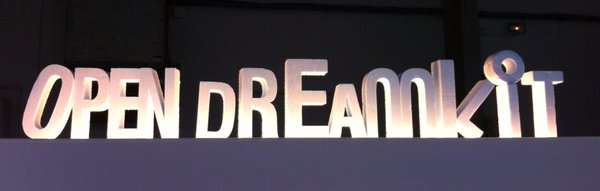
\includegraphics[scale=0.3]{pictures/kickoff1.jpg}
    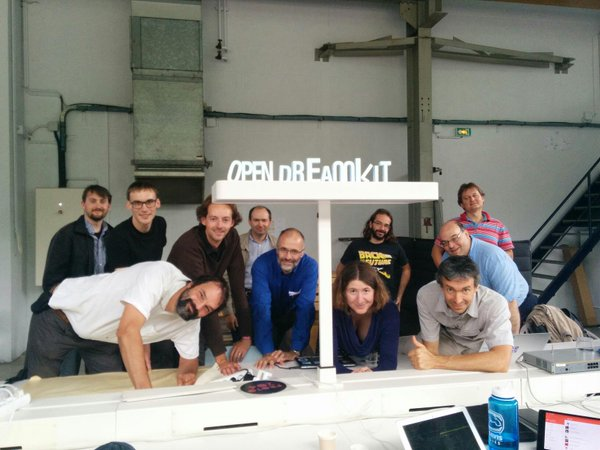
\includegraphics[scale=0.5]{pictures/kickoff2.jpg}
  \end{figure}
\end{event}
